\chapter{Theory of neutrino physics}\label{sec:NeutrinoTheory}
%%%%%%%%%%%%%%%%%%%%%%%%%%%%%%%%%%%%%%%%%%%%%%%%%%%%%%%%%%%%%%%%%%%%%%%%%%%%%%%
%%% 1. Brief history up to neutrinos being in the SM

Neutrinos were first theoretically proposed by Wolfgang Pauli \cite{PauliNeutrinoProposalLetter.pdf,TheIdeaOfTheNeutrino.pdf} as very light electrically neutral particles with a half-spin and a possible magnetic moment \cite{NeutrinoMagMomentImplications1934.pdf}. They formed a crucial part of Enrico Fermi's successful theory of $\beta$ decays \cite{FermisTheoryOfBetaDecayOriginal.pdf, FermisTheoryOfBetaDecay.pdf}, which solidified their importance in particle physics even before their first experimental detection.
Fermi's theory developed into the \gls{SM} of particle physics \cite{SMGlashow.pdf,SMWeinberg.pdf,SMSalam.pdf}, which in its current form contains three generations of fermions. Each generation consists of two leptons, one charged lepton and one neutrino, which has no mass, nor magnetic moment.

The \gls{SM} is mathematically described by a Lagrangian, in which neutrinos are represented by a two-component left-handed chiral fields $\nu_{\alpha L}$, where $\alpha=e,\mu,\tau$ denotes the three neutrino generations, also called flavours \cite{LandauParityViolationForNus.pdf, LeeYangNuAsMasslessWeylSpinor.pdf, SalamNuAsMasslessWeylSpinors.pdf}. Neutrino fields form weak isospin doublets $L_\alpha =\begin{pmatrix}\nu_{\alpha_L}\\ \alpha_{_L}\end{pmatrix}$ with their associated left-handed charged lepton fields $\alpha_L$. Unlike for the charged leptons, there is no right-handed chiral neutrino singlet field in the \gls{SM}. This means that neutrinos cannot obtain a mass term, since the fermion mass terms arise from the Higgs mechanism \cite{HiggsMechanismOriginal1964.pdf, HiggMechanismEnglertBrut1964.pdf, HiggsMechanismGuralnikHagenKibble1964.pdf} via the Yukawa coupling of the fermion and the Higgs fields\footnote{Further discussion about possible neutrino mass terms in Sec.~\ref{sec:NuMass}} \cite{YukawaLagrangiaWeinberg1967.pdf}, which requires a combination of left-handed and right-handed chiral fields \cite{FundamentalsOfNeutrinoPhysics.pdf}. Additionally, since neutrinos are massless in the \gls{SM}, all the neutrinos are left-handed helicity particles, and all the antineutrinos $\left(\overline{\nu}\right)$ are right-handed helicity antiparticles. Neutrinos and antineutrinos are mutually related by \gls{CP} symmetry: $\nu\xleftrightarrow{CP}\overline{\nu}$.

%\cite{FundamentalsOfNeutrinoPhysics.pdf} Physical neutrinos and antineutrinos are related by a CP transformation which interchanges neutrinos with antineutrinos and reverses helicity: $\nu\longleftrightarrow\overline{\nu}$ with CP (in the case of Majorana neutrinos, where the C transformation coincides with the identity, it is conventional to call neutrinos the states with negative helicity and antineutrinos the states with positive helicity)

%\cite{FundamentalsOfNeutrinoPhysics.pdf} In the SM, the mass of fermions arises as a result of the Higgs mechanism through the presence of Yukawa couplings of the fermion fields with the Higgs doublet. ... a fermion mass term must involve a coupling of left-handed and right-handed fileds, so it is clear that in the SM neutrinos are massless, because their fields do not have a right-handed components

The interaction terms for neutrinos can be separated into two parts, describing the \gls{CC} interactions with the $W_\mu$ gauge field and the \gls{NC} interaction with the $Z_\mu$ gauge field, which create/annihilate the $W^\pm$ and $Z^0$ gauge bosons respectively. Neglecting the non-neutrino components, the two neutrino interaction terms are \cite{FundamentalsOfNeutrinoPhysics.pdf}
\begin{equation}\label{eq:NuIntCCLagrangian}
\mathcal{L}_{\textsc{CC}}^{\textsc{SM}}=
-\frac{g_w}{\sqrt{2}}\sum_{\alpha=e,\mu,\tau}\overline{\nu}_{\alpha L}\gamma^\mu\alpha_L W_\mu^+ +\textsf{h.c.}\,\,\,\textsf{and}
\end{equation}
\begin{equation}\label{eq:NuIntNCLagrangian}
\mathcal{L}_{\textsc{NC}}^{\textsc{SM}}=
-\frac{g_w}{2\cos\left(\theta_W\right)}\sum_{\alpha=e,\mu,\tau} \overline{\nu}_{\alpha L} \gamma^\mu \nu_{\alpha L} Z_\mu^0.
\end{equation}
Here $g_w$ is the weak coupling constant, $\theta_W$ is the Weinberg angle and $\gamma^\mu\,\left(\mu=0,1,2,3\right)$ are the four Dirac gamma matrices.

These two terms describe all the possible \gls{SM} neutrino interaction vertices, as shown in Fig.~\ref{fig:FeynmanNuIntVertices}. These diagrams show the \gls{CC} and the \gls{NC} interaction of neutrinos and antineutrinos and, in case of the \gls{CC} diagram, can also be flipped around the vertical axis to show the production of neutrinos from the weak interaction (or decays) of leptons. They can also be rotated $90^{\circ}$ to either show the annihilation, or the production of the neutrino-lepton (for \gls{CC}), or neutrino-antineutrino (for \gls{NC}) pairs.

\begin{figure}[hbtp]
\centering
%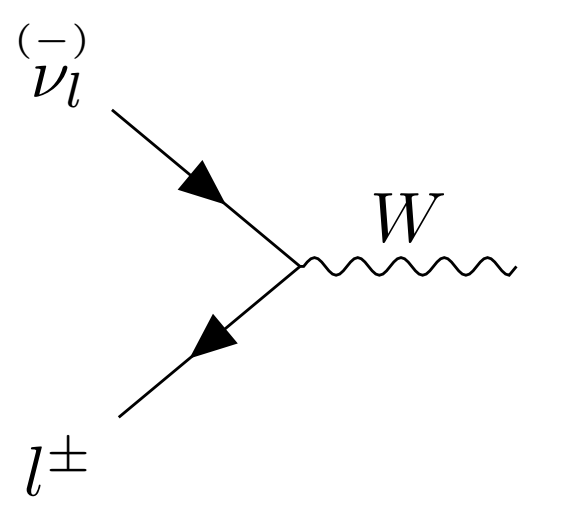
\includegraphics[height=3.2cm]{Plots/Theory/NeutrinoCCAnnihilationVertices.png}
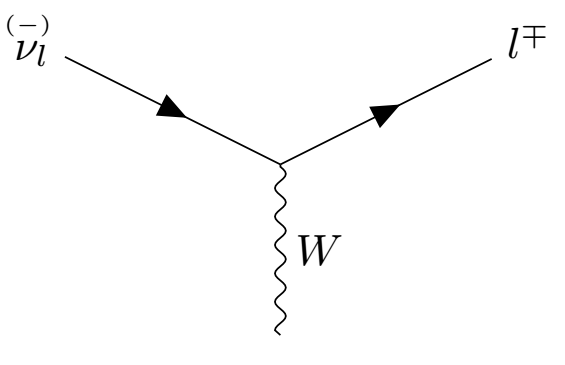
\includegraphics[width=.4\linewidth]{Plots/Theory/NeutrinoCCInteractionVertices.png}
\hspace{0.1\linewidth}
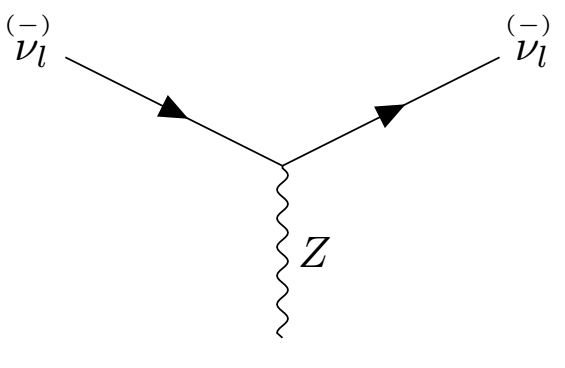
\includegraphics[width=.4\linewidth]{Plots/Theory/NeutrinoNCInteractionVertices.png}
\caption[Neutrino interaction vertices in the SM]{Neutrino interaction vertices in the \acrshort{SM} via the weak charged currents (left) and the neutral currents (right).}
\label{fig:FeynmanNuIntVertices}
\end{figure}


% in weak isospin doublets \cite{FundamentalsOfNeutrinoPhysics.pdf} grouped with their lepton left handed chiral components of charge leptons. Since SM neutrinos do not have a right handed counterpart, they can't acquire mass through the Yukawa lagrangian which combined the left and right handed fields. Their interaction lagrangian is...

%Neutrinos in the \gls{SM} are described as massless with a left-handed chiral field, with no right-handed neutrino chiral field counter part. Neutrinos make a lepton doublet together with their associated leptons. There are no neutrino mass terms in the \gls{SM} Lagrangian and the interaction terms can be divided into two types: the \gls{CC} and the \gls{NC} interactions \cite{FundamentalsOfNeutrinoPhysics.pdf}

%Neutrinos are grouped together with their corresponding charged lepton to form isospin doublets with no right handed neutrino singlet counterpart. In the SM a fermion mass term must involve a coupling of left-handed and right-handed fields and since neutrinos only have left handed fields they can't obtain

%[nuMM/nuElmagInt2015.pdf] However, there was no sign of a neutrino mass. After the discovery of parity violation in 1957, Landau (1957), Lee and Yang (1957), and Salam (1957) proposed the two-component theory of massless neutrinos, in which a neutrino is described by a Weyl spinor and there are only left-handed neutrinos and right-handed antineutrinos. It was, however, clear (Case, 1957; Mclennan, 1957; Radicati and Touschek, 1957) that two-component neutrinos could be massive Majorana fermions and that the two-component theory of a massless neutrino is equivalent to the Majorana theory in the limit of zero neutrino mass. The two-component theory of massless neutrinos was later incorporated in the standard model of Glashow (1961), Weinberg (1967), and Salam (1969), in which neutrinos are massless and have only weak interactions. In the standard model Majorana neutrino masses are forbidden by the $\textsf{SU}\left(2\right)_L\times \textsf{U}\left(1\right)_{\gamma}$ symmetry.

%[nuMM/nuElmagInt2015.pdf] In the standard model of electroweak interactions (Glashow, 1961; Weinberg, 1967; Salam, 1969), neutrinos are described by two-component massless left-handed Weyl spinors (Giunti and Kim, 2007). The masslessness of neutrinos is due to the absence of right-handed neutrino fields, without which it is not possible to have Dirac mass terms, and to the absence of Higgs triplets, without which it is not possible to have Majorana mass terms.

%[OverviewOfNeutrinoPhysicsPheno2024.pdf] three neutrino flavours produced with charged antilepton, or producing a charged lepton in CC weak interaction processes. Therefore neutrino have exhibited a polarisation in a direction that is opposite to their motion, or, equivalently, with negative helicity. For antineutrino it is the opposite. To account for this neutrino are described in the SM with a left handed chiral field $\nu_{\alpha L}\left(x\right)$. In the absence of neutrino masses, this field destroys (creates) neutrinos (antineutrinos) with negative (positive) helicity.  In the SM, neutrinos are considered massless, and no right-handed (RH) neutrino chiral field is included in its content as they would be singlet under the SM gauge group. As such, the corresponding RH neutrinos would be completely inert. Neutrinos and their lepton LH fields form SU(2) doublets $\psi_{\alpha L}\left(x\right)=\left(\nu_{\alpha L}\left(x\right),\alpha_L\left(x\right)\right)$ with hypercharge +1.

%%%%%%%%%%%%%%%%%%%%%%%%%%%%%%%%%%%%%%%%%%%%%%%%%%%%%%%%%%%%%%%%%%%%%%%%%%%%%%%
%%% 2. Neutrino production and sources
\section{Neutrino Production}
Some of the most common neutrino and antineutrino production channels include nucleon transitions via \gls{CC} weak interactions. Specifically, the transition of a neutron into a proton, either as the decay of a free neutron, or as the $\beta^-$ decay for neutrons bound in nucleus, produces an electron and an electron antineutrino:
\begin{equation}
n\rightarrow p+e^-+\overline{\nu}_e.
\end{equation}
The study of the electron spectrum from $\beta^-$ decay was the reason Pauli proposed the existence of the neutrino \cite{PauliNeutrinoProposalLetter.pdf}. Additionally, this channel is an abundant source of $\overline{\nu}_e$ from nuclear reactors, which were the first artificial sources of neutrinos, increasing the neutrino flux by about 100 million compared to the naturally occurring sources, thus enabling the first ever detection of a neutrino \cite{CowanReinesFirstAttempt.pdf, CowanReinesConfirmation.pdf, NeutrinoPhysicsCowanReines.pdf}.

Similarly, the production of an electron neutrino together with a positron via the transition of a proton into a neutron can occur inside the nucleus either as the $\beta^+$ decay:
\begin{equation}
p\rightarrow n+e^++\nu_e,
\end{equation}
or via the electron capture:
\begin{equation}
p+e^-\rightarrow n+\nu_e.
\end{equation}
This channel occurs in stars and in the first phase of supernovae \cite{FundamentalsOfNeutrinoPhysics.pdf}.

However, most supernovae neutrinos are created via a thermal pair production via \gls{NC} interaction
\begin{equation}
e^-+e^+\rightarrow\nu_\alpha+\overline{\nu}_\alpha
\end{equation}
producing neutrinos and antineutrinos of all flavours. Neutrino pair production via the decay of $Z^0$ was studied in great detail \cite{ZDecay.pdf}, since the magnitude of the $Z^0$ decay width depends on the number of neutrino flavours which can couple to $Z^0$, with the current best fit $N_\nu=2.984$ \cite{ZDecayPrecise.pdf}. Therefore, there should be exactly three light active neutrino flavours.
%Similar interactions produced the currently unobservable relic neutrinos, which were produced during the Big Bang and have extremely low energies.

%In 1990 the L3 Collaboration studied properties of the $Z^0$ boson and fitted to its peak cross-section and decay width to determine the total number of active (interacting with $Z^0$) light ($m_{\nu}<m_{Z}/2$) neutrino flavours ($N_{\nu}$). They found the best fit integer value to be 3 and ruled out the possibility of four or more active light neutrino flavours at $4\sigma$ \cite{ZDecay.pdf}. Latest most precise results put the fitted value to $N_{\nu}=2.9840\pm 0.0082$ \cite{ZDecayPrecise.pdf}.

An abundant source of $\nu_\mu$ and $\overline{\nu}_\mu$ is the decay of pions and muons
\begin{align}
p+X \rightarrow \pi^\pm \rightarrow &\mu^\pm + \nu_\mu\left(\overline{\nu}_\mu\right) \\
 & \mu^\pm \rightarrow e^\pm + \nu_\mu\left(\overline{\nu}_\mu\right) + \nu_e\left(\overline{\nu}_e\right),
\end{align}
which naturally occurs in Earth's atmosphere from the interaction of cosmic ray protons. It is notable, that if all the muons decay by the time they reach Earth's surface, the ratio of $\nu_\mu : \nu_e$ should be exactly 2:1. The same process is also used in the modern accelerator-based neutrino sources, which use protons from accelerators with desired energies, impinge them onto a fixed target, and focus the resulting hadrons to achieve a highly pure and precise source of $\nu_\mu$ or $\overline{\nu}_\mu$ \cite{GoodmanAdvancesInNeutrinoPhysics.pdf, SchwartzAccelerators.pdf}.

Similarly to $\pi$, heavier hadrons, such as kaons and charmed particles, can be produced from accelerated protons and other particles, either from natural or artificial origins. These hadrons then also produce neutrinos, including $\nu_\tau$ and $\overline{\nu}_\tau$ if their energies are high enough \cite{ObservationOfTauNeutrino.pdf, FinalTauNeutrinoResultsDONUT2008.pdf}.

%[Master's] The advent of fission reactors brought increase of neutrino rate of about $10^7$, as well as higher neutrino energies, making the neutrino detection worth reinvestigating \cite{NeutrinoPhysicsCowanReines.pdf}. In 1960 Mel Schwartz designed the first neutrino beam made by accelerated protons striking a target, producing pions (mostly), which would decay into neutrinos \cite{GoodmanAdvancesInNeutrinoPhysics.pdf}\cite{SchwartzAccelerators.pdf}.

%%%%%%%%%%%%%%%%%%%%%%%%%%%%%%%%%%%%%%%%%%%%%%%%%%%%%%%%%%%%%%%%%%%%%%%%%%%%%%%
%%% 3. Interaction of neutrinos
\section{Neutrino Interactions}
The interaction of neutrinos with matter can either be categorized based on the target, which is generally either an atomic electron or a nucleus, or the neutrino energy.

Neutrino-electron interactions occur either via elastic scattering, which result in a neutrino and an electron, or via the inverse muon (or tau) decay, which contains a muon (or tau) in the final state. Both of these interactions at the lowest order involve only free leptons and are very well theoretically understood. The elastic scattering has no energy threshold and can occur for any neutrino. On the other hand, due to the large difference between $m_e$ and $m_\mu/m_\tau$, the inverse muon decay has an energy threshold of $E_{\nu_\mu}>\unit[10.92]{GeV}$, and the inverse tau decay $E_{\nu_\tau}>\unit[3]{TeV}$ \cite{FundamentalsOfNeutrinoPhysics.pdf, NeutrinoOnElectronElScatteringTheory2003.pdf}.

%Interaction with nucleons
%By increasing their energy, neutrinos can interact with the individual nucleons bound inside the nucleus above a certain threshold \note{But this threshold doesn't really exist tbh} we can start describing the nucleus as a collection of individual, quasi-free nucleons and we can consider interaction of neutrinos on free nucleons \cite{NeutrinoIntOverview2012.pdf}. 

Neutrino-nucleus interactions can be to an extent approximated by an interaction of neutrino with its quasi-free nucleon constituents \cite{NeutrinoIntOverview2012.pdf}. These interactions can be separated into different interaction channels based on what happens to the nucleon and therefore on the resulting particles. The interaction channels depend on the neutrino incident energy, as illustrated on the case of $\nu_\mu$ \gls{CC} interactions in Fig.~\ref{fig:NuCCCrossSection}.

\begin{figure}[hbtp]
\centering
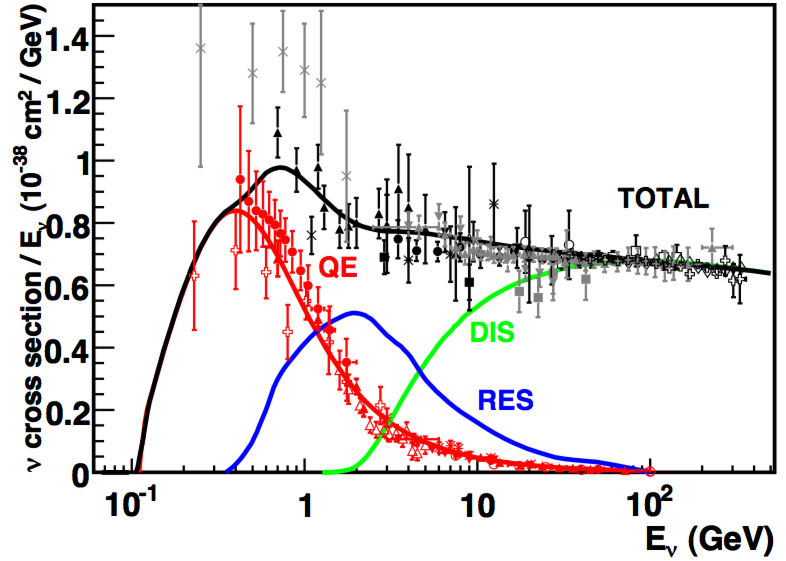
\includegraphics[width=0.8\linewidth]{Plots/Theory/NeutrinoCCCrossSections.png}
\caption[Muon neutrino CC cross sections based on the interaction types]{Neutrino \acrshort{CC} cross sections on an isolated nucleon divided by the neutrino energy based on the interaction types: \acrfull{QE}, \acrfull{Res} and \acrfull{DIS}. Figure is from \cite{NeutrinoCCCrossSectionPlot.pdf} and compares the measured data \cite{NeutrinoIntOverview2012.pdf} and the prediction provided by the NUANCE generator \cite{NuanceNuIntSimulation2002.pdf}.}
\label{fig:NuCCCrossSection}
\end{figure}

%Low energies - outcome is a single nucleon with/out lepton
At lower energies, neutrino-nucleon interactions result in the production of either a nucleon together with a neutrino in the case of \gls{NC} elastic scattering or a nucleon coupled with a charged lepton in the case of \gls{CC} \gls{QE} interactions. The \gls{CC}\gls{QE} interaction of an antineutrino on a proton
\begin{equation}\label{eq:InvBetaDecay}
\overline{\nu}_\alpha +p\rightarrow n+\alpha^+
\end{equation}
is called the inverse $\beta$ decay and was used for the first ever detection of neutrinos (specifically $\overline{\nu}_e$ from a nuclear reactor) \cite{CowanReinesFirstAttempt.pdf, CowanReinesConfirmation.pdf}. Together with the interaction of a neutrino on a neutron
\begin{equation}
\nu_\alpha+n\rightarrow p+\alpha^-
\end{equation}
they serve as fundamental processes for neutrino detection \cite{Homestake1968.pdf, MuonNeutrinoDetection.pdf, ObservationOfTauNeutrino.pdf}. The low energy threshold is based on the mass of the produced charged lepton, with no threshold for $\nu_e$ and thresholds of $E_{\overline{\nu}_e}\gtrsim\unit[1.8]{MeV}$, $E_{\nu_\mu}\gtrsim\unit[110]{MeV}$ and $E_{\nu_\tau}\gtrsim\unit[3.5]{GeV}$.

\iffalse
At lower energies neutrinos interact either via elastic interactions in the \gls{NC} channel (not shown in Fig.~\ref{fig:NuCCCrossSection}), simply knocking the nucleon out of the nucleus, or via the \gls{QE} interactions in the \gls{CC} channel, transforming the neutron or proton into its nucleon counterpart. For example, the \gls{CC}\gls{QE} interaction of an antineutrino on a proton
\begin{equation}
\overline{\nu}_\alpha +p\rightarrow n+\alpha^+
\end{equation}
is often called the inverse $\beta$ decay and was used for the first ever detection of neutrinos (specifically electron antineutrinos from a nuclear reactor) by Cowan and Reines \cite{CowanReinesFirstAttempt.pdf, CowanReinesConfirmation.pdf}. Analogically, the interaction of a neutrino on a neutron
\begin{equation}
\nu_\alpha+n\rightarrow p+\alpha^-
\end{equation}
is often used for the detection of neutrinos. It has no energy threshold for $\nu_e$ and was used for the first detection of solar neutrinos \cite{Homestake1968.pdf}. For $\nu_\mu$ the low energy threshold of \gls{CC}\gls{QE} interaction on a free nucleon is about $\unit[110]{MeV}$, which can be clearly seen in Fig.~\ref{fig:NuCCCrossSection} as the drop in the cross section at low energies. This channel is used for the detection of $\nu_\mu$, first from an accelerator \cite{MuonNeutrinoDetection.pdf} and then also for atmospheric neutrinos \cite{FirstAtmosphericNuDetIndia.pdf, FirstAtmosphericNuDetIndia2.pdf, FirstAtmNuDetectionSouthAfrica1965.pdf}. The threshold for the \gls{CC}\gls{QE} interaction of $\nu_\tau$ is about $\unit[3.5]{GeV}$, making it difficult to detect \cite{ObservationOfTauNeutrino.pdf}.
\fi

%%% Resonance production and DIS
At higher energies, neutrinos can transfer enough energy to the outgoing nucleon to excite it into a resonant baryon, which then decays back into the nucleon and into one or more additional particles. This \gls{Res} has a threshold of about $\unit[270]{MeV}$ for $\nu_\mu$ and can be distinguished by the presence of an additional $\pi$ on top of the \gls{CC}\gls{QE} products, or, at higher energies, even of multiple additional $\pi$'s or other hadrons. Increasing the neutrino incident energy even higher means that neutrinos can start probing the quark contents of the individual nucleons in the \gls{DIS}, as can be seen in Fig.~\ref{fig:NuCCCrossSection}.

%With an increase in neutrino energy above a certain threshold (about $\unit[270]{MeV}$ for $\nu_\mu$), neutrinos start the \gls{Res}. These baryons then commonly decay into a nucleon, same as for the \gls{QE} interaction, however now with additional hadrons. These hadrons are initially single pions at lower neutrino energies, but become multiple pions and other hadrons at higher energies. With even higher incident energies, neutrinos start probing the quark contents of the individual nucleons in the \gls{DIS} interaction, as can be seen in Fig.~\ref{fig:NuCCCrossSection}.

%Mention that the NC resonance production of $\pi^0$ or $\gamma$ could potentially mimic the electron signal so this can be a significant background for the nuone interactions. In the case for resonant production neutrino produces an additional hadron to the nucleon from the QE interactions...

%[NeutrinoIntForLBL2016.pdf] At energies above $\approx \unit[200]{MeV}$, the first inelastic excitations of the nucleon connected with pion production become possible. The threshold is $\unit[150.5]{MeV}$ for $\nu_e$ and $\unit[277.4]{MeV}$ for the $\nu_\mu$

%With higher energies there can be more pions and also other mesons or hyperons and so on.

%For DIS the neutrino doesn't interact with the nucleon as a whole but with its quark constituents

%%% Nuclear effects
Even though the approximation of nuclei as collections of quasi-free nucleons is useful, it has been shown \cite{MiniBooNE2p2hExperimentalDiscrepancy2010.pdf} that there are important nuclear effects that have to be considered. For example the Fermi motion of nucleons and their binding inside the nucleus, or Pauli's exclusion principle resulting in nucleon energy levels \cite{NeutrinoIntOverview2022.pdf}. Another important example is the \gls{2p2h} interaction \cite{FirstUseOfMEC2009.pdf, FirstUseOfMEC2010.pdf, FirstUseOfMEC2011.pdf}, which occurs when neutrinos interact with a correlated pair of nucleons and can significantly increase the \gls{QE} cross section \cite{NeutrinoIntOverview2022.pdf}. The \gls{2p2h} interaction often occurs via \gls{MEC}, where the meson effectively propagates the interaction between the two correlated nucleons. Furthermore, the products of all of the aforementioned interactions can re-interact inside of the nucleus in \glspl{FSI}, which can alter the particle content actually seen in the detector.

%However, recently we discovered that nuclear effect can't actually be ignored and we can't really consider neutrino nucleus interaction as a neutrino on nucleon interaction. 

%[Maria's thesis] A neutrino can interact with a pair of bound nuclei, thus knocking out two nucleons instead of one, as pictured in Figure 1.14. This is also referred as 2p2h, as the interaction leaves two holes in the struck nucleus. Most frequently, this occurs via the meson exchange current (MEC), where the two nucleons are interacting with each other via a meson.


%[Maria's thesis] The nucleons and pions and others particles can re-interact within the nucleus. Specifically for pions there are a number of processes that can happen: absorption, (quasi)elastic scattering, charge exchange,... These can also happen multiple times

%For neutrinos interacting on the nuclei, we distinguish between different types of interactions based on what happens to the nucleus. If it's an interaction with a single proton or neutron, we call this \gls{QE} interaction. If this proton gets excited into a $\Delta$ resonance (which then generally decays into a $\pi$), we call this Resonant production, if neutrino penetrates through the nucleon and interacts directly with a quark inside it, we call this \gls{DIS} interaction. This is shown on Fig.~\ref{fig:NuCCCrossSection}. There can be additional subtypes due to nuclear effects, namely the 2p2h interaction \todo{Find a reference for the 2p2h} also called \gls{MEC}, or possible \gls{FSI}.

Additionally, if the total energy transferred to the nucleus is small relative to its size, neutrinos can interact with the entire nucleus coherently, where the contributions from each individual nucleon are added together. At low energies, neutrinos can interact via the \gls{CEvNS} \cite{CEvENSFirstObservation2017.pdf}, which results in the excitation of the nucleus. At higher energies, neutrinos can interact via the \gls{COHpi} production, which produces a single $\pi$ without transferring much momentum to the nucleus. In case of the \gls{CC}\gls{COHpi} production, there is an additional charged lepton and the produced $\pi$ is positive (negative) for (anti)neutrinos, and for the \gls{NC}\gls{COHpi} production the produced $\pi$ is neutral. As the $\pi$ receives most of the transferred momentum, it generally travels in the direction of the initial neutrino and can be difficult to distinguish especially from $e$ and $\gamma$ signal in a detector \cite{NeutrinoIntOverview2022.pdf}.

%\cite{NeutrinoIntOverview2022.pdf} Also coherent meson production, in which neutrino scatters from the nucleus producing mesons but the nucleus stays in the ground state, possible via both CC and NC. The momentum transferred to the nuclear target is very small and almost all the transferred momentum is taken by the outgoing meson. The coherence condition $Q\ll 1/R$ is satisfied and the individual amplitudes for the pion production from each nucleon in the nucleus add coherently. Most of the $\pi^\pm,\pi^0$ produced (through the electromagnetic shower as their decay products) in the forward direction through the coherent reactions mimic the real $\mu^\pm$ or $e^-$ signal.

%nu-on-e is for example used for the detection of solar neutrinos in the Kamiokande experiments
%Nu-on-e is mainly sensitive to electron neutrinos, whose cross section is about 6 times larger than for the muon/tau neutrinos.

%%%%%%%%%%%%%%%%%%%%%%%%%%%%%%%%%%%%%%%%%%%%%%%%%%%%%%%%%%%%%%%%%%%%%%%%%%%%%%%
%%% Masters
%%% Experimental evidence for neutrino %%%
%Soon after Fermi's description of neutrino interaction, in 1934, Bethe and Peierls realized the possibility of reverting the process of beta decay as a mean of direct detection of the neutrino \cite{BethePeierlsDirectDetection.pdf}. For example an interaction in which incident neutrino interacts with proton, transforming it into neutron and creating a positron. From the lifetime of then-known beta decays they estimated the interaction cross-section to be $<\unit[10^{-44}]{cm^2}$ for a neutrino with a few $\unit{MeV}$ energy, or about $10^{-20}$ times the more familiar nuclear values at the time.

%In 1953 C.~L.~Cowan and F.~Reines placed a liquid scintillation detector near the Hanford reactor reporting uncertain results \cite{CowanReinesFirstAttempt.pdf}. They later moved the detector to the Savannah River Plant and in 1956 confirmed \cite{CowanReinesConfirmation.pdf} the detection of the antineutrino, verifying the neutrino hypothesis \cite{NeutrinoPhysicsCowanReines.pdf}.
%(\ovnu{$\nu$} interacting with proton, producing neutron and positron (\ovnu{$\nu$}$+p\rightarrow n+e^+$))

% Electron neutrino
%The first electron neutrino detection was by the Homestake neutrino experiment detecting solar neutrinos \cite{Homestake1968.pdf}

%%% Muon neutrino %%%
%Leon Lederman, Jack Steinberger and others joined Schwartz and using a spark chamber detector in 1962 observed \cite{MuonNeutrinoDetection.pdf} for the first time the muon neutrino $\nu_{\mu}$. Atmospheric neutrinos were first observed by the Kolar Gold Field Mine in South India \cite{FirstAtmosphericNuDetIndia.pdf, FirstAtmosphericNuDetIndia2.pdf} and in the East Rand Proprietary Gold Mine in South Africa \cite{FirstAtmNuDetectionSouthAfrica1965.pdf}.

% Tau neutrino
%After this result it was only a matter of time, before the third neutrino, the tau neutrino ($\nu_{\tau}$) was discovered. Evidence for that were shown in 2000 from the DONUT Collaboration at Fermilab \cite{ObservationOfTauNeutrino.pdf}.
%%% End of master's on neutrino history
%%%%%%%%%%%%%%%%%%%%%%%%%%%%%%%%%%%%%%%%%%%%%%%%%%%%%%%%%%%%%%%%%%%%%%%%%%%%%%%

%I think I should mention here the basic neutrino interactions and their corresponding cross section. For neutrino on nucleons, the total cross section per neutrino energy is around $\unit[0.7\times 10^{-38}]{cm^2GeV^{-1}}$ for neutrinos and half that for antineutrinos. For neutrino on electron interactions, the total cross section per neutrino energy is more similar to $10^-41-\unit[10^{-42}]{cm^2GeV^{-1}}$.

%Problems of the SM
%[OverviewOfNeutrinoPhysicsPheno2024.pdf] Besides, the SM falls short in describing other challenging issues, including the long-standing problems of explaining the nature of dark matter [12] and the overabundance of matter over antimatter in the Universe [13]. These fundamental problems may be inter-related, with neutrinos potentially playing a primary role in establishing such connections

\section{Neutrino Oscillation}
The idea that neutrinos can oscillate originates as a possibility of transitions between neutrinos and antineutrinos \cite{Pontecorvo57.pdf,Pontecorvo58.pdf}, analogically to the already known oscillations of $K^{0}\leftrightarrow \overline{K^0}$. This was adapted to the oscillations between different neutrino flavours \cite{MNS1962Osc.pdf,Pontecorvo69.pdf}, by considering that the flavour neutrino states $\nu_\alpha$, which are the eigenstates of weak interactions described in Eq.~\ref{eq:NuIntCCLagrangian} and \ref{eq:NuIntNCLagrangian}, are not identical to the mass neutrino states $\nu_k$, which are the eigenstates of the vacuum Hamiltonian $\mathcal{H}_0$:
\begin{equation}\label{eq:NuOscVacHamiltonian}
\mathcal{H}_0\ket{\nu_k}=E_k\ket{\nu_k}, k=1,2,3,...,
\end{equation}
with energy $E_k$. Instead, the neutrino flavour and mass eigenstates are related as
\begin{equation}\label{eq:NuOscFlavourMassRel}
\ket{\nu_{\alpha}}=\sum_{k} U_{\alpha k}^{*}\ket{\nu_{k}},
\end{equation}
where $U$ is the \gls{PMNS} matrix, named after the authors of neutrino oscillations \cite{FundamentalsOfNeutrinoPhysics.pdf, Gonzalez-GarciaNuMassesAndMixing.pdf}. $U$ is defined as unitary, which makes the inverse relation simply
\begin{equation}\label{eq:NuOscMassFlavourRel}
\ket{\nu_k}=\sum_\alpha U_{\alpha k}\ket{\nu_\alpha}.
\end{equation}

Using the Schr\"{o}dinger equation
\begin{equation}
i\frac{d}{dt}\ket{\nu_k\left(t\right)}=\mathcal{H}\ket{\nu_k\left(t\right)},
\end{equation}
the evolution of massive neutrino states in vacuum $\left(\mathcal{H}=\mathcal{H}_0\right)$ can be described by plane waves
\begin{equation}\label{eq:NuOscPlaneWave}
\ket{\nu_k\left(t\right)}=e^{-iE_kt}\ket{\nu_k}.
\end{equation}
The energy of a neutrino state with mass $m_k$ and momentum $\overrightarrow{p}$
\begin{equation}
E_k=\sqrt{\overrightarrow{p}^2+m_k^2}
\end{equation}
can be approximated as
\begin{equation}\label{eq:NuOscUltrarelativisticApprox}
E_k\xrightarrow{m^2\ll p^2\approx E^2}E+\frac{m_k^2}{2E},
\end{equation}
assuming small neutrinos masses and for ultra-relativistic neutrinos \cite{FundamentalsOfNeutrinoPhysics.pdf}. Additionally, as it is generally easier to measure the distance neutrinos travel $\left(L\right)$, rather than the time $\left(t\right)$, and given the notation $c\equiv 1$, where $c$ is the speed of light in vacuum, it is common to interchange $L\leftrightarrow t$.

Given the orthogonality of neutrino states, $\braket{\nu_k|\nu_j}=\delta_{kj}$ and $\braket{\nu_{\alpha}|\nu_{\beta}}=\delta_{\alpha\beta}$, and using Eq.~\ref{eq:NuOscPlaneWave}, \ref{eq:NuOscFlavourMassRel} and \ref{eq:NuOscMassFlavourRel}, the amplitude of the oscillation (transition) from $\nu_\alpha\rightarrow\nu_\beta$ over the `baseline' $L$ can be written as
\begin{equation}
A_{\nu_\alpha\rightarrow\nu_\beta}\left(L\right)\equiv\braket{\nu_\beta|\nu_\alpha\left(L\right)}= \sum_{k} U_{\alpha k}^{*} U_{\beta k} e^{-i E_kL}
\end{equation}
and the probability as
\begin{equation}
P_{\nu_{\alpha}\rightarrow\nu_{\beta}}\left( L\right) =
\left|A_{\nu_\alpha\rightarrow\nu_\beta}\left(L\right)\right|^2 =
\sum_{k, j}U_{\alpha k}^*U_{\beta k}U_{\alpha j}U_{\beta j}^*e^{-i\left(E_k-E_j\right)L}.
\end{equation}

Using Eq.~\ref{eq:NuOscUltrarelativisticApprox} and by defining the neutrino mass splitting (also called the mass squared difference) as
\begin{equation}\label{Deltamsq}
\Delta m_{kj}^{2}\equiv m_{k}^{2}-m_{j}^{2},
\end{equation}
the oscillation probability can be expressed as
\begin{equation}\label{eq:NuOscProbability}
P_{\nu_{\alpha}\rightarrow\nu_{\beta}}\left( L\right) = \sum_{k, j}U_{\alpha k}^*U_{\beta j}U_{\alpha j}U_{\beta j}^*e^{-i\frac{\Delta m_{kj}^2 L}{2E}}.
\end{equation}

%This led B. Pontecorvo, inspired by already known $K^{0}\leftrightarrow \overline{K^0}$ oscillations, to consider $\nu\leftrightarrow\overline{\nu}$ transitions (oscillations), in case the conservation of neutrino charge does not apply\cite{Pontecorvo57.pdf}. Pontecorvo later built upon this statement in 1958 considering that oscillations between $\nu$ and $\overline{\nu}$ are due to them being combinations of particles $\nu_1$ and $\nu_2$ and that the transformation lifetime is related to the mass difference between $\nu_1$ and $\nu_2$ \cite{Pontecorvo58.pdf}, laying foundation for neutrino oscillations as we know them today.

%In 1962 Z. Maki, M. Nakagawa and S. Sakata applied Pontecorvo's idea of neutrino oscillations to \textit{weak neutrino} eigenstates $\nu_{\alpha}$ ($\nu_e$, $\nu_{\mu}$) produced in weak interactions. They assumed that oscillation $\nu_{\alpha}\leftrightarrow\nu_{\beta}$ are driven by a non-zero mass difference (therefore if true implying at least one neutrino has a non-zero mass) between \textit{true neutrinos} (= mass neutrino eigenstates $\nu_i$ ($\nu_1$, $\nu_2$)), which are related to weak eigenstates via a linear combination. This relation in general case looks like \cite{MNS1962Osc.pdf}
%where $U$ is a unitary matrix now know as Pontecorvo-Maki-Nakagawa-Sakata (PMNS) matrix and $n$ is the (general) number of light neutrino species \cite{Gonzalez-GarciaNuMassesAndMixing.pdf}.

\iffalse
Oscillation probability can be also expressed as
\begin{align}\label{OscProb}
P_{\nu_{\alpha}\rightarrow\nu_{\beta}}\left( L\right)= \delta_{\alpha\beta}
& -4\sum_{i>j}\text{Re} \left( U_{\beta i}U_{\alpha i}^{*} U_{\beta j}^{*}U_{\alpha j}\right)
\sin^{2}\Delta_{ij}\nonumber \\
& +2\sum_{i>j} \text{Im} \left( U_{\beta i}U_{\alpha i}^{*}U_{\beta j}^{*}U_{\alpha j}\right) \sin 2\Delta_{ij},
\end{align}
where\cite{Gonzalez-GarciaNuMassesAndMixing.pdf} \[\Delta_{ij}\equiv\Delta m_{ij}^{2}\frac{L}{4E}=1.267\frac{\Delta m_{ij}^{2}}{\unit{eV^2}}\frac{L/E}{\unit{m}/\unit{MeV}} .\]

Since real neutrino beams are not monochromatic, what is measured in experiments is an \textbf{average} oscillation probability with $\left\langle \sin^{2}\Delta_{ij}\right\rangle$ and $\left\langle\sin2\Delta_{ij}\right\rangle $ in eq.\ref{OscProb}. We can notice that if $E/L\gg\Delta m_{ij}^{2}$ the oscillation does not show any effect yet and if $E/L\ll\Delta m_{ij}^2$ the oscillating phase goes through many cycles and is averaged to $\left\langle \sin^{2}\Delta_{ij}\right\rangle=1/2$. Therefore different experimental settings can measure different oscillation parameters \cite{PDG.pdf}.
\fi

So far no assumption has been made as to the specific number of neutrino mass or flavour states. However, as was described above, there are exactly three active neutrino flavour states, $\nu_e$, $\nu_\mu$ and $\nu_\tau$. Consequently, it is common to also consider exactly three neutrino mass states. This is often called the three neutrino paradigm. Therefore, the \gls{PMNS} matrix has size $3\times 3$ and can be written as \cite{FundamentalsOfNeutrinoPhysics.pdf}:
\[
U=
\begin{pmatrix}
 U_{e1}     & U_{e2}     & U_{e3}    \\
 U_{\mu 1}  & U_{\mu 2}  & U_{\mu 3} \\
 U_{\tau 1} & U_{\tau 2} & U_{\tau 3}
\end{pmatrix}
=\,\,\,
\]
\begin{equation}\label{param3}
\,\,\,\,\,\,\,\, =
\begin{pmatrix}
 1 & 0       & 0      \\
 0 & c_{23}  & s_{23} \\
 0 & -s_{23} & c_{23}
\end{pmatrix}
\begin{pmatrix}
 c_{13}              & 0 & s_{13}e^{-i\delta} \\
 0                   & 1 & 0                  \\
 -s_{13}e^{i\delta} & 0 & c_{13}
\end{pmatrix}
\begin{pmatrix}
 c_{12}  & s_{12} & 0 \\
 -s_{12} & c_{12} & 0 \\
 0       & 0      & 1
\end{pmatrix},
\end{equation}
where $c_{ij}\equiv\cos\theta_{ij}$ and $s_{ij}\equiv\sin\theta_{ij}$. The matrix is parametrized using three mixing angles $\theta_{12}$, $\theta_{13}$ ,and $\theta_{23}$ and one phase, often denoted $\delta_{CP}$. The phase describes a possible \gls{CP} symmetry violation in neutrino oscillations, which would result in a difference between the neutrino and antineutrino oscillation probabilities.
%Specifically, $\delta_{CP}$ different from $N\pi$, where $N\in\mathbb{Z}$, would imply \gls{CP} symmetry violation, which in turn results in a difference between neutrino and antineutrino oscillations.
% and the other two are $\alpha$ and $\beta$, so called Majorana phases, which are non zero only if neutrinos are Majorana (neutrinos and antineutrinos are described by just one field, i.e. neutrinos are the same particle as antineutrinos). Majorana phases play no role in neutrino oscillations, so they are usually left out in the description \cite{PDG.pdf}. The PMNS matrix in this case can be parametrized as

%%% Matter effect
%The hamiltonian in Eq.~\ref{eq:NuOscVacHamiltonian} and all the previous considerations only consider neutrino oscillations in vacuum, without possible interactions in matter. 
When neutrinos pass through matter, their evolution changes due to coherent elastic \gls{CC} and \gls{NC} scattering. However, since the \gls{NC} scattering affects all neutrino flavours equivalently, it does not have any effect on neutrino oscillations. Additionally, as electrons are the only charged leptons present in matter, only the relative difference between the \gls{CC} interactions of $\nu_e$ and of other flavours needs to be considered. The effective interaction potential of neutrinos passing through matter with an electron density $N_e$ can be written as
\begin{equation}
V_{\textsc{CC}}=\pm\sqrt{2}G_{F}N_{e}.
\end{equation}
Here $G_F$ is the Fermi coupling constant and the plus or minus sign is for neutrinos or antineutrinos respectively. The electron density (and therefore the interaction potential) can change along the neutrino path, as it does in the Sun, which can resonantly increase the probability of oscillations, as described by the \gls{MSW} effect \cite{Wolfenstein78.pdf, MikheyevSmirnov85.pdf}. However, in accelerator based experiments, where neutrinos only pass through the surface of the Earth, the $N_e$ can be described as approximately constant.

The effect of neutrinos passing through matter on oscillation probabilities can be expressed as shifts to mixing angles and to mass squared differences, proportional to the $V_{\textsc{CC}}$. Since the matter effect differs for neutrinos and antineutrinos, it needs to be carefully considered especially for the $\delta_{CP}$ measurement, which relies on the comparison of neutrino to antineutrino oscillations \cite{FundamentalsOfNeutrinoPhysics.pdf}.

\iffalse
To consider the effect of neutrinos passing through matter on neutrino oscillations, now also called the \gls{MSW} effect \cite{Wolfenstein78.pdf, MikheyevSmirnov85.pdf}, we have to include the interaction hamiltonian
\begin{equation}
\mathcal{H}=\mathcal{H}_0+\mathcal{H}_I.
\end{equation}
effect of which can be described by a potential
\begin{equation}
\mathcal{H}_I\ket{\nu_\alpha}=V_\alpha\ket{\nu_\alpha}.
\end{equation}
This interaction potential $V_\alpha$ is different for $\nu_e$ compared to the other flavours, as $\nu_e$ can have \gls{CC} interaction with electrons, which are highly abundant in the universe unlike the other charged leptons \cite{FundamentalsOfNeutrinoPhysics.pdf}. In a simple form, we can express it as
\begin{equation}
V_\alpha=V_{\textsc{CC}}\delta_{\alpha e}+V_{\textsc{NC}}=
\pm\sqrt{2}G_{F}\left(N_{e}\delta_{\alpha e}-\frac{1}{2}N_n\right),
\end{equation}
where $G_F$ is the Fermi coupling constant, $N_e$ is the electron density, $N_n$ is the neutron density and the plus and minus sign is for neutrinos and antineutrinos respectively.

This effect of this potential on the neutrino oscillation probability can effectively be understood as shifts to the values of the mixing angles and the mass squared differences. Size of the shifts depends on the matter neutrinos pass through and the shifts are in the opposite direction for neutrinos and antineutrinos. This means that the \gls{MSW} effects needs to be carefully considered especially for the measurement of the $\delta_{CP}$, which rely on the comparison of neutrino to antineutrino oscillations.
\fi
%This potential is different for neutrinos and antineutrinos! Matter effect can help us distinguish the sign of the $\Delta m^2$ and the octant of $\theta$! However, since it's also different for neutrinos and antineutrinos it can either increase the difference caused by the $\delta_{CP}$, or can go in the opposite direction, depending on the individual values.

%The matter effect for neutrino oscillations is a result of an imbalance between the interaction probability of $\nu_e$ and $\nu_{\mu}/\nu_{\tau}$, due to the abundance of electrons in matter. 

\iffalse
%%%%%%%%%%%%%%%%%%%%%%%%%%%%%%%%%%%%%%%%%%%%%%%%%%%%%%%%%%%%%%%%%%%%%%%%%%%%%%%
%%% Master's on matter effect
Possible explanation of the Solar neutrino problem was proposed in 1978 by L. Wolfenstein, who considered the effect of matter on neutrino oscillations \cite{Wolfenstein78.pdf}. His modification of neutrino oscillations when passing through matter arises from the coherent forward scattering of electron neutrinos, as a result of their charged current (CC) interaction with electrons, which are abundant in matter, as opposed to other lepton flavours, muons and tauons, resulting in an imbalance between $\nu_e$ and $\nu_{\mu}/\nu_{\tau}$. This manifests as an effective potential, which depends on the density and composition of the matter \cite{Wolfenstein78.pdf}. This idea was later further developed for neutrinos passing through the Sun by Mikheyev and Smirnov in 1985 \cite{MikheyevSmirnov85.pdf}\cite{Gonzalez-GarciaNuMassesAndMixing.pdf} and we now call this effect the Mikheyev-Smirnov-Wolfenstein (MSW) effect.

To showcase this effect we consider only two neutrino flavours, $\nu_e$ and $\nu_X$, where $X$ denotes a combination of all other non-electron flavours. Vacuum oscillations are in this two-neutrino approximation driven by a single mass splitting $\Delta m^2$ and the corresponding PMNS matrix is a rotational matrix parametrized by one angle $\theta$:
\begin{equation}
U=
\begin{pmatrix}
 \cos\theta  & \sin\theta    \\
 -\sin\theta & \cos\theta
\end{pmatrix}.
\end{equation}

This potential can be seen as having the effect of modifying the $\Delta m^2$ and $\theta$ of the neutrino oscillations: \cite{CERNSchool2001.pdf}
\begin{equation}\label{MSWEffect}
\sin^22\theta_m=\frac{\sin^22\theta}{\sin^22\theta+\left(\cos 2\theta\mp\xi\right)^2}
\end{equation}
\begin{equation}
\left(\Delta m^2\right)_{\textsl{eff}}=\Delta m^2\times\sqrt{\sin^22\Theta+\left(\cos 2\theta\mp\xi\right)^2},
\end{equation}
where 
\begin{equation}
\xi=\frac{2\sqrt{2}G_FN_e}{\Delta m^2}.
\end{equation}
\fi
%%% End of master's on neutrino oscillations
%%%%%%%%%%%%%%%%%%%%%%%%%%%%%%%%%%%%%%%%%%%%%%%%%%%%%%%%%%%%%%%%%%%%%%%%%%%%%%%

%Experimental evidence that lead to neutrino oscillations
The first experimental signs of neutrino oscillations appeared as an apparent deficit of solar neutrinos compared to their predicted flux \cite{Homestake1968.pdf}. However, due to low confidence in the prediction of the solar neutrino flux, no conclusion could have been drawn. Similarly, experiments measuring atmospheric neutrinos \cite{NUSEX89.pdf, Frejus95.pdf, IMP92.pdf, Kamiokande94.pdf} saw a disagreement between the measurement and the prediction for the $\nu_\mu : \nu_e$ fraction of the atmospheric neutrino flux. This \textit{atmospheric neutrino anomaly} was finally resolved by the \gls{SK} experiment \cite{EvidenceForAtmoOscFirstEverOscRes.pdf}, reporting the first experimental evidence for neutrino oscillations. The \textit{solar neutrino anomaly} was resolved shortly after by the \gls{SNO} experiment \cite{NCOscInSNOSecondOscResult.pdf}, which compared the \gls{NC} rate, unaffected by neutrino oscillations, to the rate of \gls{CC} neutrino interactions. This was proof that solar neutrinos oscillate without reliance on the model of the Sun. This result also confirmed the importance of accounting for the matter effect in neutrino oscillations, especially for the oscillation of solar neutrinos, due to the large matter density in the Sun.

%Neutrino oscillations were suggested as an explanation for the observed deficit of solar neutrinos \cite{Homestake1968.pdf} and for the disagreement between the measurement and the prediction for the $\nu_\mu : \nu_e$ fraction of the atmospheric neutrinos \cite{NUSEX89.pdf, Frejus95.pdf, IMP92.pdf, Kamiokande94.pdf}. The so-called atmospheric neutrino anomaly was resolved by the \gls{SK} experiment \cite{EvidenceForAtmoOscFirstEverOscRes.pdf}, which reported the first evidence for neutrino oscillations. The solar neutrino anomaly was resolved by the \gls{SNO} experiment \cite{NCOscInSNOSecondOscResult.pdf}, which compared the rate of the \gls{CC} interaction, which are affected by neutrino oscillations, and of the \gls{NC} interaction, which can't determine between neutrino flavours and are therefore unaffected by neutrino oscillations. The results from \gls{SNO} also confirmed that we need to account for the \gls{MSW} effects, especially for solar neutrinos, due to the large $N_e$ in the Sun.

%[Master's] Several experimental indications for neutrino oscillations were found shortly after its theoretical predictions. Already in 1968 their Homestake Solar Neutrino Observatory saw a solar neutrino flux less than 3 Solar Neutrino Units (SNU = one interaction per $10^{36}$ target atoms $\unit{s^{-1}}$), well below the solar model prediction of the time \cite{Homestake1968.pdf}. This discrepancy became the \textit{“solar neutrino problem”}, which is in line with neutrino oscillations, but no direct implications could have been drawn since it might have been caused by a lack of understanding of nuclear physics, astrophysics of the Sun, or particle physics of the neutrino\cite{GoodmanAdvancesInNeutrinoPhysics.pdf}. Kamiokande experiment, which confirmed the results from Homestake \cite{Kamiokande96.pdf}.

%The Solar neutrino anomaly was also resolved, when the Sudbury Neutrino Observatory (SNO) provided $>5\sigma$ evidence for  solar $\nu_e$ oscillations in 2002, independent on the solar model \cite{NCOscInSNOSecondOscResult.pdf}. While other solar neutrino experiments measured solar $\nu_e$ only via the charged current (CC) interactions SNO had an ability to also detect neutrinos via the neutral current (NC) interaction which are equally sensitive to all active neutrino flavours and their rate is therefore unaffected by standard neutrino oscillations. SNO could compare CC and NC event rates and conclude that $\nu_e$ from the Sun oscillate into other neutrino flavours along the way \cite{NCOscInSNOSecondOscResult.pdf}.

%Atmospheric neutrino experiments - atmospheric neutrino anomaly - how many neutrinos
%Measuring atmospheric neutrinos brought about another neutrino conundrum, the \textit{Atmospheric neutrino anomaly}. It came from the disagreement between experiments such as NUSEX\cite{NUSEX89.pdf} and Fr\'{e}jus\cite{Frejus95.pdf}, which used iron calorimeters detectors, and experiments IMP\cite{IMP92.pdf} and Kamiokande\cite{Kamiokande94.pdf}, which used water Cherenkov detectors. All of these experiments were looking for a deficit of $\nu_{\mu}$, or an excess of $\nu_e$, compared to prediction. While the first two experiments saw a good agreement between experimental results and predictions, the latter two did not and suggested the possibility of neutrino oscillations, which could explain their disagreement. Solution to the Atmospheric neutrino anomaly came in 1998, when the Super-Kamiokande (SK) experiment showed for the first time the~experimental evidence for neutrino oscillations \cite{EvidenceForAtmoOscFirstEverOscRes.pdf}. SK has however also disfavoured the two neutrino hypothesis, with regards to the existence of an additional neutrino flavour. 

The difference between the frequency of solar neutrino oscillations and that observed in atmospheric neutrinos proves that there are at least two mass splittings governing neutrino oscillations. As a result, there must be at least three separate neutrino mass states, with at least two of them possessing non-zero masses. This is in direct contradiction to the \gls{SM} and is to-date the only laboratory-based observation of physics \gls{BSM} \cite{SnowmassNeutrinoFrontierReport.pdf}.

%\cite{IUPAP_Neutrino_Panel_Report_2021.pdf} These observations, subsequently confirmed using neutrinos produced in nuclear reactors and at accelerator facilities, established that the three-flavor oscillations of Eq. (4) can be described to a good approximation by two, decoupled oscillations. The first, describing the oscillations of atmospheric muon neutrinos, is characterized by a large mass-squared difference and a mixing angle that is approximately 45 degrees. The second, describing the oscillations of solar electron neutrinos, is characterized by a small mass-squared splitting and a large (approx. 35 degrees) mixing angle. $\theta_{23}$ is referred to as the “atmospheric mixing angle” as it determines at leading order the oscillations of atmospheric muon neutrinos while $\theta_{12}$ is referred to as the solar mixing angle as it is used, at leading order, to describe the oscillations of solar electron neutrinos. The mixing angle $\theta_{13}$ is small, accounting for the approximate decoupling of the atmospheric and solar oscillations. For Majorana neutrinos there are two additional phases (“Majorana phases”), which an be put in a diagonal phase matrix to the right of Eq.(5). See Sec. 5.3 for a discussion. Two additional phases that might arise if neutrinos are Majorana particles can not be measured in neutrino-oscillation experiments and are omitted from Eq. (5). 

%%% History and current state of neutrino oscillation measurements
%From Eq.~\ref{eq:NuOscProbability}, we can see that the frequency of neutrino oscillations depends on the $\Delta m^2$. In case of three neutrino mass states, there are two independent mass squared differences.  Other than the PMNS matrix, neutrino oscillations depend on the mass squared differences (eq.\ref{Deltamsq}). In case of 3 neutrinos, those are $\Delta m^2_{21}$ and $\Delta m^2_{31}$. $\Delta m^2_{21}$ mainly drives oscillations of solar neutrinos and is therefore often denoted as $\Delta m^2_{\odot}$ or $\Delta m^2_{sol}$, while $\Delta m^2_{31}$ drives oscillations on the scale for atmospheric neutrinos  and is often written as $\Delta m^2_{atm}$ \cite{Gonzalez-GarciaNuMassesAndMixing.pdf}. \todo{Update this and mention that this means that there must be at most one massless neutrino states and neutrinos must have mass}

Currently, the three neutrino paradigm of oscillations between three neutrino flavour states via three neutrino mass states is well established \cite{PDG.pdf, NuOscGlobalFit2020.pdf}. The magnitudes of both the neutrino mass splittings and of two mixing angles, $\theta_{12}$ and $\theta_{13}$, are measured within $3\%$. The third mixing angle $\theta_{23}$ is measured to be close to the maximum mixing value of $45^{\circ}$. However, there are three main questions yet to be determined for neutrino oscillations \cite{SnowmassNeutrinoFrontierReport.pdf}:
\begin{enumerate}
\item What is the sign of the larger neutrino mass splitting? Is the electron neutrino made up of the lightest neutrino mass states (normal ordering), or the heaviest (inverted ordering)?
\item Is $\theta_{23}<45^{\circ}$ or $\theta_{23}>45^{\circ}$? These determine the $\nu_\mu : \nu_\tau$ relative contributions to the neutrino mass states and are also referred to as the upper and the lower octant respectively.
\item Is there \gls{CP} violation in neutrino oscillations? What is the value of $\delta_{CP}$? If neutrinos oscillate differently than antineutrinos, this could be an important part of the matter-antimatter asymmetry in the Universe.
\end{enumerate}
All three of these questions are jointly investigated in the current \gls{LBL} accelerator neutrino oscillation experiments, namely the \gls{NOvA} \cite{NOvAResults2021.pdf} and the \gls{T2K} \cite{T2KOscResults2023.pdf} experiments. Both use precise $\accentset{(-)}{\nu}_\mu$ beams, affected by the matter effect, and compare the rates of
$\accentset{(-)}{\nu}_\mu$ disappearance and $\accentset{(-)}{\nu}_e$ appearance to constrain neutrino oscillation parameters \cite{SnowmassNeutrinoFrontierReport.pdf}. The same methods will be used in the next generation \gls{LBL} neutrino oscillation experiments, the \gls{DUNE} \cite{IntroductionToDUNE2020.pdf} and the \gls{HK} \cite{HyperKTDR2018.pdf}, which should give the final answers to all three neutrino oscillation questions \cite{SnowmassNeutrinoFrontierReport.pdf}.
 
% (2.8\% and 1.1\%), as well as the size of two mixing angles, $\theta_{12}$ and $\theta_{13}$ (2.3\% and 1.4\% and 2.4\%)

%The absolute values (magnitudes) of the two neutrino mass splitting are well measured, two of the mixing angles are known fairly well $\theta_{13}$ and $\theta_{12}$ and for the third $\theta_{23}$ we know it is close to the maximum, but still trying to figure out whether it is $<45^{\circ}$ or $>45^{\circ}$, also called the octants. We still don't know what is the $\delta_{CP}$ \cite{SnowmassNeutrinoFrontierReport.pdf}.

%$\delta_{CP}$ could help explain the matter antimatter asymmetry in the universe. The fact that the Universe consists of matter and not antimatter hints at a fundamental asymmetry between matter and antimatter, in the form of CP violation. We know that the known sources of CP violation via quark mixing and from the QCD Lagrangian are insufficient to account for the composition of the Universe. Neutrino oscillation is sensitive to one new CP phase and if neutrinos are Majorana particles, there are two additional neutrino-sector CP phases which may contribute to matter-antimatter asymmetry \cite{SnowmassNeutrinoFrontierReport.pdf}. 

%[IUPAP_Neutrino_Panel_Report_2021.pdf] Neutrinos oscillate which implies that leptons mix in analogy to quarks. This means that neutrinos have non-vanishing rest masses, which requires at least one new particle species beyond the ones in the standard model.

%[IUPAP_Neutrino_Panel_Report_2021.pdf] The size of the matter effect depends on the density and composition of the medium and on the oscillation parameters. In particular, the matter effect may be exploited to determine the octant of the mixing angles and the sign of the mass-squared differences. Moreover, the matter effect is different for neutrinos and antineutrinos because for the latter A changes sign. The difference between the oscillation probabilities of neutrinos and antineutrinos that arises from the matter effect must be taken into account in searches for CP-invariance violation. The CP-invariance violation arising from $\delta_{CP}$ must be distinguished from that which arises due to the matter effect. This can be accomplished by exploiting the differences in the modulations of the four oscillation probabilities $\nu_e$ appearance, $\overline{\nu}_e$ appearance, $\nu_\mu$ disappearances and $\overline{\nu}_\mu$ disappearance.

\section{Neutrino Mass}\label{sec:NuMass}
%%% Neutrino mass measurements and Dirac definitions
%Need to say that masses cant be measured in neutrino oscillation experiment, that the measurement comes from the kinematic imbalance and that the current limits put the masses well below the masses of other fermions.
The absolute values of neutrino masses are currently not known and cannot be directly measured in neutrino oscillation experiments. Results from experiments measuring the kinematic distribution of $\beta$ decays \cite{KATRINFirstSubeVNuMassResult.pdf}, or from cosmology \cite{PlanckResultsNuMadd2020.pdf}, set a limit for each neutrino mass to $<\unit[1]{eV}$. This is several orders of magnitude smaller than the charged fermion masses, suggesting that theories \gls{BSM} which introduce neutrino masses should have a different mechanism for their generation than the one used for the other fermions \cite{PDG.pdf}. Furthermore, in order to introduce neutrino masses into the \gls{SM}, it is necessary to either add new fields, break the renormalizability of the \gls{SM} Lagrangian, or do both \cite{Gonzalez-GarciaNuMassesAndMixing.pdf}.
%The only model-independent information on the size of neutrino masses comes from measurements of missing energy in reactions involving a neutrino. The current best limit on the effective mass of $\nu_e$ (a combination of neutrino mass states via neutrino oscillation parameters) is $m_{\nu_e}<\unit[0.8]{eV/c^2}$ at 90\% C.L. \cite{KATRINFirstSubeVNuMassResult.pdf}. The overall best limit on neutrino masses comes from cosmology, placing a limit on the sum of neutrino masses $\sum_a m_a <\left(0.12-0.69\right)\unit{eV/c^2}$ at 95\% C.L. \cite{PlanckResultsNuMadd2020.pdf}. This limit however depends on the cosmological model \cite{PDG.pdf}. These are significantly smaller than the mass scales of other fermions, suggesting a different theoretical mechanism for their generation.

%The theoretical mechanism that generates neutrino masses is currently not known and is directly connected to the question on the nature of neutrinos. So far we have only considered neutrinos to be Dirac particles. This means that... And the most trivial neutrino mass generation mechanism, also called the minimally extended \gls{SM}, add three right handed Dirac neutrinos. This is not used as it doesn't explain the smallness of neutrino masses. 
%[OverviewOfNeutrinoPhysicsPheno2024.pdf] The most stringent upper bound on the sum of neutrino masses comes from observations of the Cosmic Microwave Background by PLANCK [71], combined with supernovae and other cosmological and astrophysical data, yielding $\sum_a m_a <\left(0.12-0.69\right)\unit{eV}$ at 95\% C.L. depending on the adopted cosmological model and level of statistical complexity [72, 73] (see also [74–78]).

%%% Dirac masses and their problems
The most straight-forward solution, often called the \textit{minimally extended \gls{SM}}, is to add the missing right-handed chiral neutrino fields, which would enable neutrino mass generation through Yukawa couplings with the Higgs field. These right-handed fields would however be singlets under all the \gls{SM} gauge symmetries and would therefore not participate in any of the \gls{SM} interactions. Neutrinos created by these fields are called \textit{sterile} and could potentially mix with the \textit{active} neutrinos via neutrino oscillations. There are however a few issues with the minimally extended \gls{SM}. Since the mass generation mechanism is the same as for the charged fermions, there is no theoretical explanation for the relative smallness of neutrino masses. There is also currently no experimental confirmation of oscillations between active and sterile neutrinos \cite{PDG.pdf}, although there are some possible indications \cite{LSND2001.pdf, MiniBooNE2018.pdf}. Additionally, having to add new fields by hand makes the \gls{SM} an incorrect description of reality even at low energies. This is an issue, as it is generally believed that \gls{SM} is at least a good low energy  effective theory of a more complex general theory and only breaks down at some \gls{NP} threshold value $\Lambda_{NP}$ \cite{Gonzalez-GarciaPhenomenologyMassiveNu.pdf}.

%This is however one of the largest limitations of this simple extension of the \gls{SM}. Since the neutrino masses are so different from other fermions, it is unlikely their mass generation is the same as for the other fermions. The minimally extended \gls{SM} gives no explanation about the smallness of neutrino masses. Furthermore, this simple extension would render \gls{SM} incorrect even at low energies, even though it is generally believed that \gls{SM} is an effective low-energy extrapolation of a generally correct theory, that break at some threshold value of \gls{NP} $\Lambda_{NP}$ \cite{Gonzalez-GarciaPhenomenologyMassiveNu.pdf}. Additionally, there was no oscillation between active and light sterile neutrinos detected to date.

%Sterile neutrinos have none of the SM gauge interactions and they are singlets of the full SM gauge group. As discussed above, with the fermionic content and gauge symmetry of the SM one cannot construct a renormalizable mass term for the neutrinos. So in order to introduce a neutrino mass one must either extend the particle contents of the model or abandon gauge invariance and/or renormalizability. \cite{Gonzalez-GarciaNuMassesAndMixing.pdf}

%\cite{PDG.pdf} [for Dirac neutrinos only] Let us stress that in this case both the low-energy matter content and the assumed symmetries are different from those of the SM. Consequently, the SM is not even a good low-energy effective theory. Furthermore, this scenario does not explain the fact that neutrinos are much lighter than the corresponding charged fermions, because all of them acquire their mass via the same mechanism.

\iffalse
[Fundamentals of neutrino physics and astrophysics] The only extension of the SM that is needed is the introduction of right-handed components $\nu_{\alpha R}$ of the neutrino fields. Such a model is sometimes called the \textit{minimally extended Standard Model}. The right handed neutrino fields are fundamentally different from the other elementary fermion fields because they are invariant under the symmetries of the SM: they are \textbf{singlets} of $\textsf{SU}(3)_C\times\textsf{SU}(2)_L$ and have hypercharge $Y=0$. The right handed neutrino fields are called sterile [883 = B. Pontecorvo, Sov. Phys. JETP, 26, 984-988, 1968] because they do not participate in weak interactions and their only interaction is gravitational. their right handedness is not required though! could also be left handed but have to be singlets and therefore sterile!

In the minimally extended standard model with three right handed neutrino fields, the SM Higgs-lepton Yukawa Lagrangian is extended by adding a lepton term with the same structure as the second term on the right handed side, which generates the masses of up-type quarks
\begin{equation}
\mathcal{L}_Y=
-\sum_{\alpha,\beta=e,\mu,\tau} Y_{\alpha\beta}^{\prime l} \overline{L}_{\alpha L}\Phi l_{\beta R}^{\prime}
-\sum_{\alpha,\beta=e,\mu,\tau} Y_{\alpha\beta}^{\prime \nu} \overline{L}_{\alpha L}\tilde{\Phi} \nu_{\beta R}^{\prime}
+\textsf{h.c.},
\end{equation}
where $Y^{\prime \nu}$ is a new matrix of Yukawa couplings.

Using the unitary gauge we can diagonalize the Yukawa couplings we obtain
\begin{equation}
\mathcal{L}_Y=
-\sum_{\alpha=e,\mu,\tau}\frac{y_\alpha^l v}{\sqrt{2}}\overline{l}_\alpha l_\alpha
-\sum_{k=1}^N \frac{y_k^\nu v}{\sqrt{2}}\overline{\nu}_k\nu_k
-\sum_{\alpha=e,\mu,\tau}\frac{y_\alpha^l}{\sqrt{2}}\overline{l}_\alpha l_\alpha H
-\sum_{k=1}^N \frac{y_k^\nu}{\sqrt{2}}\overline{\nu}_k\nu_k H
\end{equation}

Therefore the neutrino masses are given by
\begin{equation}
m_k=\frac{y_k^\nu v}{\sqrt{2}}\,\,\,\left(k=1,...,N\right),
\end{equation}
and massive Dirac neutrinos couple to the Higgs field through the last term. Note that the neutrinos masses are proportional to the Higgs VEV $v$, as the masses of charged leptons and quarks. However, it is known that the masses of neutrinos are much smaller than those of charged leptons and quarks, but there is no explanations here of the very small values of the eigenvalues $Y_k^{\nu}$ of the Higgs-neutrino Yukawa coupling matrix that are needed. The lagrangian defined this way does not conserve the lepton flavour number, which leads to neutrino oscillations. The Dirac character of massive neutrinos is closely related to the invariance of the total Lagrangian under the global U(1) gauge transformations.
\fi

%\cite{Gonzalez-GarciaPhenomenologyMassiveNu.pdf} In case of only Dirac neutrinos $\left(M_N=0\right)$ Let’s point out that in this case the SM is not even a good low-energy effective theory since both the matter content and the assumed symmetries are different. Furthermore there is no explanation to the fact that neutrino masses happen to be much lighter than the corresponding charged fermion masses as in this case all acquire their mass via the same mechanism.

%%% Majorana particles definition
Adding new non-renormalizable terms to the \gls{SM} Lagrangian which are suppressed by this \gls{NP} scale as $1/\Lambda_{NP}$, would maintain the renormalizability (and validity) of the \gls{SM} at energies well below $\Lambda_{NP}$ \cite{Gonzalez-GarciaPhenomenologyMassiveNu.pdf}. It is possible to create such a term using only the existing \gls{SM} fields and preserving the \gls{SM} gauge symmetries, which after spontaneous symmetry breaking generates neutrino mass terms. Additionally, three of the newly generated masses are also suppressed as $1/\Lambda_{NP}$ and belong to mostly left-handed (active) fields, while the rest are very large $\left(\sim\Lambda_{NP}\right)$ and belong to mostly sterile neutrinos, which are therefore also called \glspl{HNL}. This is called the see-saw mechanism \cite{SeeSawMechanism1979.pdf} and provides a natural explanation for the smallness of neutrino masses. Furthermore, the heavy masses of \gls{HNL} make them more likely to avoid experimental detection. However, neutrinos with masses produced by this mechanism are all Majorana particles \cite{MajoranaOriginalPaper.pdf}. This means that neutrinos are their own antiparticles
\begin{equation}
\nu\equiv\nu^C,
\end{equation}
where $C$ denotes charge conjugation. This is possible for neutrinos, since they are electrically neutral, unlike the other fermions. It also means that neutrinos can effectively annihilate with each other, violating the total lepton number by two units. The antineutrinos that were described in the previous sections are still different particles to neutrinos, but in this case only differ by parity transformation. \todo{Mention Dirac neutrinos and that Majorana neutrinos have two more phases in the PMNS matrix}

%Furthermore, if \gls{SM} is only an effective theory, we could add non-renormalizable terms to the \gls{SM} Lagrangian, which would be suppressed by the scale of some \gls{NP} $\Lambda_{NP}$ \cite{Gonzalez-GarciaPhenomenologyMassiveNu.pdf}. We can add a non-renormalizable dimension five term from the field contents of the \gls{SM}, that conserves the gauge symmetries of the \gls{SM}, and after the spontaneous symmetry breaking creates a neutrino mass term, that is exactly proportional to the mass term from the see-saw model. The scale of the neutrino masses is suppressed by $1/\Lambda_{NP}$. Therefore, this would not require addition of any new fields, would explain the smallness of neutrino masses and would make the \gls{SM} a correct effective field theory at energies $E\ll \Lambda_{NP}$. The only requirement is that neutrinos are Majorana particles.
%if neutrinos are Majorana, we do not even have to add any new fields into the \gls{SM}. If we add a new non-renormalizable term into the \gls{SM} Lagrangian, that is suppressed with respect to $\Lambda_{NP}$, after spontaneous symmetry breaking leads to the exact same case with Majorana sterile neutrinos, with the masses of the light active neutrinos being suppressed by $\Lambda_{NP}$ with respect to the masses of the other fermions. This would explain the observed smallness of neutrino masses and would also mean that \gls{SM} is an effective theory of more full theory that breaks down at $\Lambda_{NP}$.

%All these issues could be solved if neutrinos are Majorana particles \cite{MajoranaOriginalPaper.pdf}, for which the right-handed chiral fields are equal (up to a phase) to the charge conjugation of the left-handed chiral fields $\nu_R = \nu_L^C$ (and vica-versa) and therefore the $\nu=\nu_L+\nu_R=\nu_L+\nu_L^C$. $\nu_L^C$ is right-handed, but transforms as $\nu_L$. This would mean that neutrinos are equivalent to antineutrinos $\nu=\nu^C$ \cite{Gonzalez-GarciaPhenomenologyMassiveNu.pdf} and what we called antineutrinos so far, would only differ from neutrinos by its chirality. This is possible, as neutrinos do not have any electric charge. This means that neutrinos can unlike for charged fermion, neutrinos can have mass terms that combine purely left, or purely right handed chiral fields as $\nu_L^T C^\dagger\nu_L$ and $\nu_R^T C^\dagger\nu_R$. This also means that we can have interactions that do not conserve the total lepton number, which is not a fundamental symmetry of the \gls{SM} and only arises as an accidental symmetry. This would allow us to create additional mass terms, either by adding a Higgs triplet into the \gls{SM} and keeping neutrino fields left-handed, or by adding $N$ right-handed chiral neutrino fields, same as in the Dirac case. These new Majorana masses are different from the Dirac masses described above. We can develop a theory which contains both Dirac and Majorana mass terms and if the $M_M\gg M_D$, then diagonalization of the mass matrix leads to three very light neutrinos with masses $\sim 1/M_M$, which are mostly left-handed, and $N$ very heavy sterile neutrinos with masses $\sim M_M$. This is called the \textit{see-saw mechanism} \cite{SeeSawMechanism1979.pdf} and it would provide a natural explanation to the smallness of neutrino masses.
%All the other massive fermions are described by Dirac spinors, but since neutrinos do not have an electric charge, they could be described as Majorana. Majorana derived a theory, where he describe fermions without antifermions, simply by  postulating that particles are their own antiparticles, therefore $\nu=\nu^C$, where $\nu^C$ is the charge-conjugate of $\nu$. Therefore, if neutrinos are Majorana, what we called antineutrinos so far, would only differ from neutrinos by its chirality. This would allow for an additional neutrino mass term with different masses than for the Dirac neutrinos, let's call them Majorana masses. This is either doable with only left-handed neutrino fields, but would require a new Higgs triplet, or with an addition of right-handed fields. For both of these cases, Majorana neutrinos violate the total lepton number.



%Since neutrinos have mass they can no longer be theoretically describe by Weyl spinors. They can be described by either Dirac of Majorana spinors. The question of neutrino mass is intrinsically connected to the question of the theoretical nature of neutrinos. This is in turn related to the question of the conservation of the total lepton number, which is preserved in the \gls{SM}. if neutrinos are majorana particles then they can also have majorana masses.


%So far we only considered neutrinos to be Dirac particles, for which particles and antiparticles are different, same as all the other fermions. 

%[Fundamentals of neutrinos physics and astrophysics,p.190] The majorana condition can be written as $\nu=\nu^C$, which implies the equality of particle and antiparticle. As noted already by Majorana [765 = E. Majorana, Nuovo Cim., 14, 171-184, 1937], since a Majorana spinor has only two independent components, the Majorana theory is simpler and more economical than the Dirac theory. Hence, the Majorana nature of massive neutrinos may be more natural than the Dirac nature. In fact, neutrinos are majorana particles in most theories beyond the SM. If the neutrino is massless, since the left handed chiral component of the neutrino field obeys the Weyl equation in both the Dirac and Majorana descriptions and the right handed chiral component is irrelevant for neutrino interactions, the Dirac and Majorana theories are physically equivalent. From this it is clear that in practice one can distinguish a Dirac from a Majorana neutrino only by measuring some effect due to the neutrino mass. Moreover, the mass effect must not be of kinematical nature, because the kinematical effects of Dirac and Majorana masses are the same. For example, the Dirac and Majorana nature of neutrinos cannot be revealed through neutrino oscillations! The most promising way to find if neutrinos are Majorana particles is the search for neutrinoless double beta decay.
%We cannot create Majorana mass terms with only left handed neutrino fields since there is no weak isospin triplet in the SM and therefore there is no renormalizable term in the SM Lagrangian which can generate Majorana mass

%[Master thesis] A new type of neutrino was suggested by Ettore Majorana in his paper on “Symmetrical Theory of Electron and Positron” [352], published in 1937, but most probably already developed a few years before [144]...Majorana suggested in his paper that the neutron or the neutrino, or both, were particles of this type, namely neutral particles which identify themselves with the corresponding antiparticles. (FromNeutronToNuclearFission.pdf)

%[Master thesis] In 1937, however, probably after being invited by Fermi to compete for a full professorship, Majorana published what was to become his most famous paper:  “Symmetric theory of electrons and positrons,” in which he introduced the so-called Majorana neutrino hypothesis.  A consequence of this theory is that a neutral fermion can coincide with its antiparticle:  This hypothesis was revolutionary because it argued that the antimatter partner of a given matter particle could be the particle itself.  And this was in direct contradiction to what Dirac had successfully assumed in order to solve the problem of negative energy states in quantum field theory (i.e., the existence of the positron).But Majorana  was just interested among the others in  eliminating the “Dirac sea” postulate...Anyway, with unprecedented farsightedness Majorana suggested that the  neutrino, which had just been postulated, as we know, by Pauli and Fermi, could be such a particle. This would make the neutrino unique among the elementary particles and, moreover, enable it to have mass:  a property that favoured the possibility of neutrino oscillations (a phenomenon,  predicted by B.Pontecorvo, and later on experimentally verified). After that Fermi made neutrinos the  basis  of  an  impressive,  quantitative  theory  of  beta  decay,it became interesting to reconsider whether one could have spinning particles that are their own antiparticles.  Could one, specifically, have a version of the Dirac equation that involved real fields?  This was a mathematical question asked, and answered, by Majorana.The exceptional theory of neutrinos by Majorana would lead us too far, and we are glad to be able to confine ourselves to refer the reader to the excellent presentations of it in works like [14,31], and refs.  therein. Let us only stress that, even if the important experiments presently performed all over the world (e.g., in USA, Japan, Italy,...)  haven’t revealed yet if neutrinos are Dirac’s or Majorana’s, nevertheless, in condendsed matter physics,  structures have been found several times that are “Majorana fermions”:  see Refs.[34-36]. (MajoranaNeutronEtNeutrino.pdf)

%[OverviewOfNeutrinoPhysicsPheno2024.pdf] ...In contrast, the Majorana phases do not enter the flavour neutrino oscillation probabilities [22, 85], but contribute to the $\left(\beta\beta\right)_{0\nu}$-decay rate (see Sec. 3.3).


%%% General case of dirac plus majorana masses - see-saw model
%We can include both Dirac and Majorana mass terms in a way, where we would naturally get three very light neutrinos and N very heavy neutrinos. This is called the see-saw model and it would provide a natural explanation to the smallness of neutrino masses. 

%If neutrinos can have both Dirac and Majorana masses, then we can have mass terms in the Lagrangian in which the additional sterile neutrinos interact with with the active neutrinos (this is the case for purely Dirac neutrinos), but can also interact with their own antineutrinos, generating Majorana masses. If we add $m$ sterile neutrinos, we get $m$ heavy sterile neutrinos and 3 light active neutrinos, which are mostly left handed. Both the light and the heavy neutrinos are Majorana particles.


\iffalse
With the particle contents of the SM and the addition of an arbitrary m number of sterile neutrinos one can construct two types mass terms that arise from gauge invariant \textbf{renormalizable} operators:
\begin{equation}
-\mathcal{L}_{M_\nu} = M_{D_{ij}}\overline{\nu}_{si}\nu_{Lj}+	
\frac{1}{2}M_{N_{ij}}\overline{\nu}_{si}\nu_{sj}^C+\textsf{h.c.},
\end{equation}
where $\nu^C$ indicated a charge conjugated field, $\nu^C=C\overline{\nu}^T$ and $C$ is the charge conjugation matrix. $M_D$ is a complex $m\times 3$ matrix and $M_N$ is a symmetric matrix of dimension $m\times m$. First term is the Dirac term generated from Yukawa interactions after spontaneous electroweak symmetry breaking. The second term in Eq. (10) is a Majorana mass term. It is different from the Dirac mass terms in many important aspects. It is a singlet of the SM gauge group. Therefore, it can appear as a bare mass term. Furthermore, since it involves two neutrino fields, it breaks lepton number by two units.

\cite{Gonzalez-GarciaPhenomenologyMassiveNu.pdf} In case of $M_N\gg M_D$ (see-saw model), The diagonalization of $M_\nu$ leads to three light, $\nu_\alpha$ , and m heavy, $N$, neutrinos, where the heavy states are mostly right-handed while the light ones are mostly left-handed. Both the light and the heavy neutrinos are Majorana particles. Two well-known examples of extensions of the SM that lead to a see-saw mechanism for neutrino masses are SO(10) GUTs [25–27] and left-right symmetry [28]. This is the see-saw mechanism [24–28]. In this case the SM is a good effective low energy theory. Indeed the see-saw mechanism is a particular realization of the general case of a full theory which leads to the SM with three light Majorana neutrinos as its low energy effective realization as we discuss next.

\cite{Gonzalez-GarciaPhenomenologyMassiveNu.pdf} In general, if the SM is an effective low energy theory valid up to the scale $\Lambda_{NP}$ , the gauge group, the fermionic spectrum, and the pattern of spontaneous symmetry breaking of the SM are still valid ingredients to describe Nature at energies $E\ll \Lambda_{NP}$. We need to consider also non-renormalizable higher dimensional terms in the lagrangian. In this approach the largest effects at low energy are expected to come from dim= 5 operators.  Indeed, there is a single set of dimension-five terms that is made of SM fields and is consistent with the gauge symmetry, and this set violates the spontaneous symmetries of the SM. It is given by
\begin{equation}
\mathcal{O}_5=\frac{Z^\nu_{ij}}{\Lambda_{NP}}\left(\overline{L}_{Li}\tilde{\Phi}\right)\left(\tilde{\Phi}^T L_{Lj}^C\right)+\textsf{h.c.},
\end{equation}
which violate total lepton number by two units and leads, upon spontaneous symmetry breaking, to:
\begin{equation}
-\mathcal{L}_{M_\nu}=\frac{Z^\nu_{ij}}{2}\frac{v^2}{\Lambda_{NP}}\overline{\nu}_{Li}\nu_{Lj}^C+\textsf{h.c.}.
\end{equation}
 we see that this is a Majorana mass term built with
the left-handed neutrino fields and with:
\begin{equation}
\left(M_\nu\right)_{ij}=Z^{\nu}_{ij}\frac{v^2}{\Lambda_{NP}}
\end{equation}

\cite{Gonzalez-GarciaPhenomenologyMassiveNu.pdf} Since Eq. (29) would arise in a generic extension of the SM, we learn that neutrino masses are very likely to appear if there is NP. As mentioned above, a theory with SM plus m heavy sterile neutrinos leads to three light mass eigenstates and an effective low energy interaction of the form (27). In particular, the scale $\Lambda_{NP}$ is identified with the mass scale of the heavy sterile neutrinos, that is the typical scale of the eigenvalues of $M_N$. ...the scale of neutrino masses is suppressed by $v/\Lambda_{NP}$ when compared to the scale of charged fermion masses providing an explanation not only for the existence of neutrino masses but also for their smallness. Finally, this supports lepton mixing and CP violation unless additional symmetries are imposed on the coefficients $Z_{ij}$.
\fi

%%% neutrinoless double beta decay
%If neutrinos are Majorana particles, they can effectively annihilate with each other and therefore violate the lepton number by two units. 
A sure way of finding out whether neutrinos are Majorana particles or not is an observation of a neutrino-less double $\beta$ decay \cite{Gonzalez-GarciaPhenomenologyMassiveNu.pdf}. This is currently a subject of an extensive experimental investigation without a concrete conclusion \cite{PDG.pdf}. Neutrinos being Majorana particles does not affect neutrino oscillations, however, other measurement could probe the nature of neutrinos, or possible theories \gls{BSM}, such as the measurements of the possible neutrino magnetic moment \cite{SnowmassNeutrinoFrontierReport.pdf}.

%Whether neutrinos are Dirac or Majorana particles can only be detected via a kinematic interactions, such as the neutrino-less double $\beta$ decay, where the two neutrinos from a standard double $\beta$ decay can annihilate as they are their own antiparticles. This is currently a subject of an extensive experimental investigation. Additionally, if neutrinos are Majorana, there would be two additional \gls{CP} violating phases in the \gls{PMNS} matrix. These would however not contribute to neutrino oscillation probabilities, but would contribute to the neutrinoless double beta decay, which is currently still being investigated. If neutrinos are Majorana, it would not affect any current measurements, but it would be of profound importance to the possible theories \gls{BSM}. There are other neutrino properties that could probe the nature of neutrinos and the possible physics \gls{BSM}, but would not be affected by oscillations, such as measuring the possible neutrino magnetic moment \cite{SnowmassNeutrinoFrontierReport.pdf}.

%Detection of neutrinoless double beta decay is the only known method with plausible sensitivity to the Majorana nature of the neutrino, one of the most important open questions in particle physics. \cite{SnowmassNeutrinoFrontierReport.pdf}

%[OverviewOfNeutrinoPhysicsPheno2024.pdf] In contrast, the Majorana phases do not enter the flavour neutrino oscillation probabilities [22, 85], but contribute to the $\beta\beta_{0\nu}$ decay rate

%[Master thesis] Another question which was studied was whether the neutrino was truly a Dirac particle in the same sense as in an electron. The formalism for `single' beta decay is indifferent to the answer, but in the case of `double' beta decay in which the simultaneous emission of two electrons occurs the situation was somewhat altered. Here the requirement that the neutrino must obey the Dirac electron equations as for `electrons' but with zero charge, and that there exist particle ($\nu$)-antiparticle ($\overline{\nu}$) pairs, resulted in very long half lives for double beta decay, whereas if the neutrinos emitted in positron decay and negative electron decay are identical, the lifetimes should be short and observable. The original work of Firemen (1948) on double beta decay stimulated many subsequent searches with the conclusion based on the presently unobservably great lifetimes that the neutrino can best be described as a `true' Dirac particle, i.e., by the Dirac equation, and that the neutrino is distinct from the antineutrino. (NeutrinoPhysicsCowanReines.pdf)

%[OverviewOfNeutrinoPhysicsPheno2024.pdf]  From the best existing lower bounds on the $\left(\beta\beta\right)_{0\nu}$-decay lifetimes of 136 Xe [68] and 76 Ge [69] one can obtain a bound on neutrino masses, which, however, applies only if neutrinos have a Majorana nature [70]: $m_{1,2,3}\leq \unit[0.58]{eV}$.

%The disparity of mass scales between neutrinos and other fundamental particles suggests a high-energy scale for neutrino-mass generation. In models where this mechanism lies at or below the TeV scale, the physics of neutrino mass may be accompanied by complementary signatures at colliders. In models where the scale is higher, experiments probing the nature of neutrino mass are the only feasible way of exploring this new physics. The observation of neutrino-less double beta decay would provide direct evidence that lepton number is violated, opening a path to baryogenesis via leptogenesis in the early universe. As such, direct tests of the scale or nature of neutrino mass target some of the most central open questions in fundamental physics today. Other neutrino properties may be connected to extensions of the standard model, yet are not observable via oscillations. Neutrino electromagnetic properties are of fundamental interest, \cite{SnowmassNeutrinoFrontierReport.pdf}.